\section{Casi d'uso}
In seguito ad un'analisi approfondita del capitolato, ad un incontro con il proponente \Zucchetti e ad una discussione tra gli Analisti, sono emersi i seguenti casi d'uso.\\
Ogni caso d'uso è identificato da un codice univoco che ne rappresenta anche la posizione all'interno della gerarchia; il codice è così composto:
\begin{center}
UC[codice rappresentante il padre].[codice progressivo]
\end{center}
Il codice progressivo può avanzare nei livelli di gerarchia divindendo tali livelli con un punto.

\newpage

%   TEMPLATE NUOVO CASO D'USO
%\subsection{Caso d'uso UC#: Descrizione}

%\begin{figure}[h]
%	\begin{center}
%	\includegraphics[scale=0.4]{diagram/UC#.png}
%	\caption{Caso d'uso UC#}
%	\end{center}
%\end{figure}

%\begin{itemize}
%	\item \textbf{Attori:} 
%	\item \textbf{Precondizioni:}
%	\item \textbf{Postcondizioni:}
%	\item \textbf{Scenario principale:}
%	\item \textbf{Estensioni:}
%\end{itemize}


\subsection{Caso d'uso UC0}

\begin{figure}[h]
	\begin{center}
	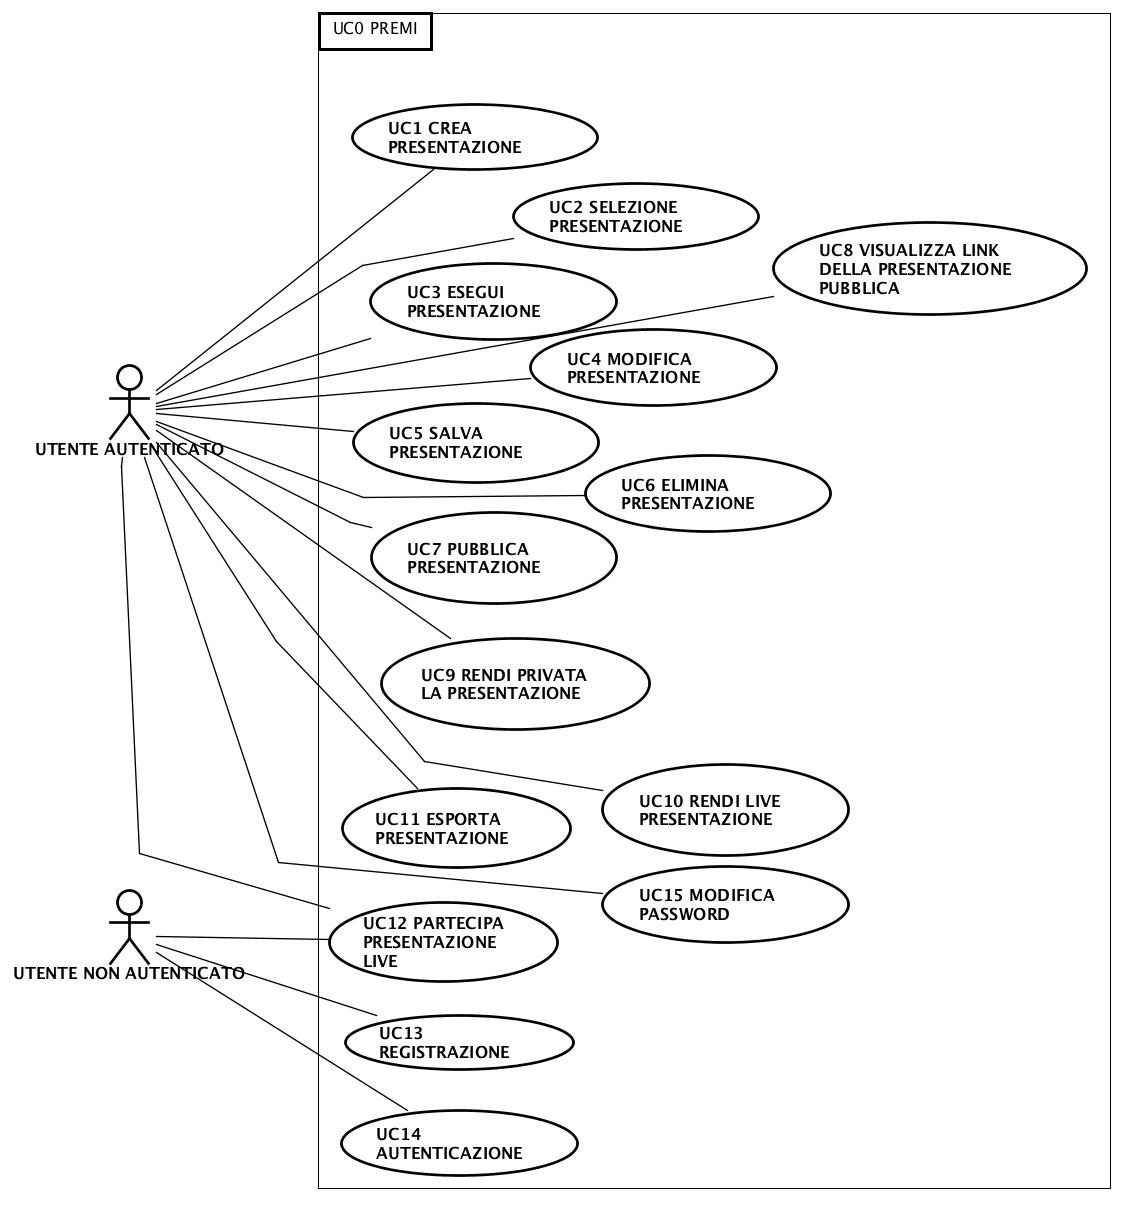
\includegraphics[scale=0.4]{diagram/UC0.png}
	\caption{Caso d'uso UC0}
	\end{center}
\end{figure}

\begin{itemize}
	\item \textbf{Attori:} Utente registrato; 
	\item \textbf{Precondizioni:}
	\item \textbf{Postcondizioni:}
	\item \textbf{Scenario principale:}
	\item \textbf{Estensioni:}
\end{itemize}

\subsection{Caso d'uso UC1}

\begin{figure}[h]
	\begin{center}
	\includegraphics[scale=0.4]{diagram/UC1.png}
	\caption{Caso d'uso UC1}
	\end{center}
\end{figure}

\begin{itemize}
	\item \textbf{Attori:} Utente registrato; 
	\item \textbf{Precondizioni:}
	\item \textbf{Postcondizioni:}
	\item \textbf{Scenario principale:}
	\item \textbf{Estensioni:}
\end{itemize}
